\chapter{\label{ch:6}Regulation of Kir6.2 by SUR1} 

\graphicspath{{figures/ch6/}}

\minitoc

\section{Introduction}
The SUR1 subunit exerts a number of different regulatory effects on the K\ATP{} channel.
Firstly, it dramatically enhances trafficking of Kir6.2 to the cell membrane by masking the endoplasmic retention motif in Kir6.2 (RKR).
Without coexpression with SUR1, Kir6.2 is confined to the endoplasmic reticulum.
Truncating the C-terminal by deleting the last 26 (Kir6.2-\textgreek{D}C26) or 36 (Kir6.2-\textgreek{D}C36) amino acids \cite{tucker_truncation_1997}, mutation of the RKR motif to AAA \cite{zerangue_new_1999}, or addition of a C-terminal GFP tag \cite{john_sulphonylurea_1998} are sufficient to allow expression of Kir6.2 at the membrane alone without the presence of SUR1.
Comparing the function of these modified Kir6.2 subunits alone to the function of octameric K\ATP{} channels makes it possible to discern the multifaceted roles of SUR1.
Crucially, these C-terminal modifications do not appear to alter K\ATP{} function when they are coexpressed with SUR1 \cite{tucker_truncation_1997, john_sulphonylurea_1998, ribalet_atp-sensitive_2006} and the cryo-EM structure solved for C-terminally GFP labelled Kir6.2 \cite{li_structure_2017} was highly similar to those solved without the GFP label \cite{martin_anti-diabetic_2017-1, lee_molecular_2017-1}.

Coexpression of SUR1 has two effects on K\ATP{} channel function.
Firstly, SUR1 increases the $P_O$ of the channel \cite{tucker_truncation_1997, john_sulphonylurea_1998, chan_n-terminal_2003-1}.
Expressing the TMD0 region of SUR1 (residues 1 - 195) alone is sufficient to recapitulate the increase in $P_O$ observed when full-length SUR1 is coexpressed\cite{babenko_sur_2003-1, chan_n-terminal_2003-1}.
When TMD0 is coexpressed with Kir6.2, there is additionally a decrease in the sensitivity of Kir6.2 to nucleotide inhibition - allosterically, an increase in $P_O$ would result in a decrease in apparent ATP affinity due to the reduction in stability of the closed state.
However, when full length SUR1 is coexpressed with Kir6.2, there is a marked increase in sensitivity to ATP inhibition \cite{tucker_truncation_1997, john_sulphonylurea_1998, chan_n-terminal_2003-1, ribalet_atp-sensitive_2006}.
This increase in sensitivity has been suggested to be not due to the L0 linker, the other domain of SUR1 postulated to make contacts with Kir6.2.
Expression of TMD0-L0 (residues 1 - 232) with Kir6.2 increases the $P_O$ to nearly saturating, and reduces ATP inhibition even further \cite{babenko_sur_2003-1}.
Increasing the fraction of L0 (up to residue number 256 or 288) attenuates this increase in $P_O$, but there is not the dramatic increase in ATP sensitivity observed from expression of full-length SUR1, implicating a role for the core region of SUR1 in regulating nuclelotide binding and inhibition \cite{puljung_cryo-electron_2018}.

In this chapter, we aim to clarify the role of SUR1 in regulating the inhibitory effect of nucleotides on K\ATP{} channel function.

\section{Intrinsic effects of SUR1}

\subsection{SUR1 dramatically alters nucleotide inhibition, but only subtly effects nucleotide binding}
Expressing WT-GFP alone without SUR1 results in smaller, noisier currents than when coexpressed with SUR1.
Currents are less sensitive to ATP and TNP-ATP by an order of magnitude (Figure \ref{ch6fig:nosur_atp}, \ref{ch6fig:nosur_tnpatp}.
Our surface expression assay suggested that while WT-GFP was able to reach the membrane in the absence of SUR1, W311*-GFP was not, and when we excised patches from cells expressing W311*-GFP alone, we were not able to resolve any currents (Figure \ref{ch3fig:surface_expression_2}).
We were still able to resolved fluorescence in unroofed membranes expressing W311*-GFP alone, and so we measured binding of TNP-ATP to W311*-GFP alone in unroofed membranes.
We observed very minimal differences in the EC\textsubscript{50} for binding.
However, given that we did not observe currents under these experimental conditions, we cannot determine the functional state of these channels and so this finding may not be representative for K\ATP{} channels physiologically.

Given that we were able to observe currents in the absence of SUR1, we confirmed that when SUR1 was cotransfected with our constructs we were measuring currents and fluorescence from correctly assembled K\ATP{} channels.
Firstly, we used tolbutamide to inhibit excised patches from cells expressing either WT-GFP alone, WT-GFP+SUR1 or W311*-GFP+SUR1.
Tolbutamide inhibition occurs at two sites on the K\ATP{} channel; a high affinity site on SUR1 and a low affinity site on Kir6.2 \cite{gribble_tissue_1998, ashfield_identification_1999}.
Inhibition occurring at these two sites can be well separated, with the high affinity site saturating at \SI{100}{\micro\Molar} tolbutamide at \SI{50}{\percent} fractional inhibition.
Tolbutamide inhibition of Kir6.2 expressed alone does not display inhibition until concentrations of over \SI{100}{\micro\Molar}.
When we expressed WT-GFP alone, we saw no inhibition of currents by \SI{100}{\micro\Molar}, whereas when we expressed WT-GFP+SUR1 or W311*-GFP+SUR1, we observed roughly a \SI{50}{\percent} fractional inhibition of current as expected for proper associated of Kir6.2 and SUR1.

\begin{figure}[h]
	\centering
	\begin{subfigure}[t]{0.35\textwidth}
		\caption{}\label{ch6fig:nosur_atp}
		\centering
		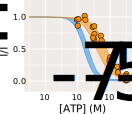
\includegraphics[width=\textwidth]{nosur_atp.pdf}
	\end{subfigure}
	\hfill
	\begin{subfigure}[t]{0.35\textwidth}
		\caption{}\label{ch6fig:nosur_tnpatp}
		\centering
		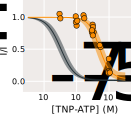
\includegraphics[width=\textwidth]{nosur_tnpatp.pdf}
	\end{subfigure}
	\vfill
	\begin{subfigure}[t]{0.35\textwidth}
		\caption{}\label{ch6fig:nosur_unroofed}
		\centering
		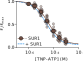
\includegraphics[width=\textwidth]{nosur_unroofed.pdf}
	\end{subfigure}
	\hfill
	\begin{subfigure}[t]{0.45\textwidth}
		\caption{}\label{ch6fig:tolb_inhibition_1}
		\centering
		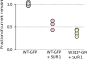
\includegraphics[width=\textwidth]{tolb_inhibition_1.pdf}
	\end{subfigure}
	\vfill
	\begin{subfigure}[t]{0.9\textwidth}
		\caption{}\label{ch6fig:nosur_ec50s}
		\centering
		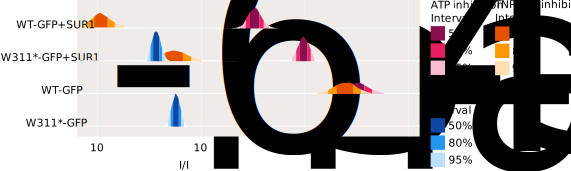
\includegraphics[width=\textwidth]{nosur_ec50s.pdf}
	\end{subfigure}
	\caption[SUR1 dramatically alters inhibition but only subtly alters binding at Kir6.2]{
	\subref{ch6fig:nosur_atp}, \subref{ch6fig:nosur_tnpatp} Current inhibition of WT-GFP expressed alone in excised patches by ATP (\subref{ch6fig:nosur_atp}) or TNP-ATP (\subref{ch6fig:nosur_tnpatp}) is shown in orange.
	The smooth filled curves are the \SI{95}{\percent} intervals of the posterior probability distribution of fits to equation \ref{eq:hill} as described in the methods.
	The blue curve is the fit to the WT-GFP+SUR1 current inhibition by ATP (\subref{ch6fig:nosur_atp}) or TNP-ATP (\subref{ch6fig:nosur_tnpatp}) and is shown for comparison.
	\subref{ch6fig:nosur_unroofed} Fluorescence quenching of W311*-GFP expressed alone by TNP-ATP in unroofed membrane patches.
	Each point represents an individual experiment.
	The smooth filled curves are the \SI{95}{\percent} intervals of the posterior probability distribution of fits to equation \ref{eq:hill} as described in the methods.
	The blue curve is the fit to the W311*-GFP+SUR1 fluorescence quenching by TNP-ATP and is shown for comparison.
	\subref{ch6fig:tolb_inhibition_1} Inhibition by \SI{100}{\micro\Molar} tolbutamide of currents from WT-GFP expressed alone (grey) or with SUR1 (blue) or from W311*-GFP expressed with SUR1 (orange).
	Each point represents an individual patch.
	\subref{ch6fig:nosur_ec50s} Posterior probability distributions for the estimated population $IC_{50}$ or $EC_{50}$ values are shown in purple ($IC_{50}$ for ATP inhibition), orange ($IC_{50}$ for TNP-ATP inhibition), or blue ($EC_{50}$ for TNP-ATP binding in unroofed membranes).
	Each distribution is shaded with respect to its intervals.
	}\label{ch6fig:no_sur}
\end{figure}

While tolbutamide inhibition provides evidence for SUR1 association with our Kir6.2 constructs in excised patches, we cannot perform the same experiment to test for association in unroofed membranes.
Instead, we labelled the C-terminus of SUR1 with the fluorophore mOrange (SUR1-mO), and measured FRET between the GFP attached to WT-GFP or W311*-GFP and the mOrange attached to SUR1.
The cryo-EM structures suggest a distance between the C-termini of Kir6.2 and SUR1 of roughly \SI{60}{\angstrom}, while the GFP-mOrange FRET pair has a theoretical R0 of \SI{54}{\angstrom}.
We would therefore expect to see FRET between GFP and mOrange if our Kir6.2 and SUR1 contructs are coassembling.

To measure FRET, we used an approach outlined by \citeauthor{clegg_18_1992} and \citeauthor{selvin_13_1995} whereby FRET is measured as an increase in the emission of the acceptor fluorophore (mOrange) on excitation of the donor fluorophore (GFP) (Figure \ref{sur_assays}).
We can directly excite both GFP and mOrange with \SI{490}{\nano\metre} light.
When WT-GFP is expressed alone we can measure the resulting emission spectrum as the donor fluorescence alone, and when SUR1-mO is expressed alone we can measure the resulting emission spectrum as the acceptor fluorescence alone (Figure \ref{ch6fig:gfp_mo_spectra_1}).
In addition, we can excite mOrange directly with \SI{565}{\nano\metre} light and avoid excitation of GFP.
However, in the experimental condition with both WT/W311*-GFP and SUR1-mO, excitation with \SI{490}{\nano\metre} light results in an emission spectrum which is a mixture of three components: the emission from the donor fluorophore GFP, emission from the acceptor fluorophore mOrange due to direct excitation, and emission from the acceptor fluorophore mOrange due to energy transfer from the donor GFP (Figure \ref{ch6fig:wt_gfp_mo_spectra_1}, \ref{ch6fig:w311_gfp_mo_spectra_1}).
To extract the component we are interested in (emission due to energy transfer), we can first remove the contribution of the donor fluorescence to the emission spectrum by subtracting an idealised WT/W311*-GFP spectrum averaged from multiple cells expressing it alone (Figure \ref{ch6fig:wt_gfp_mo_spectra_2}, \ref{ch6fig:w311_gfp_mo_spectra_2}).
We can then take the ratio of the fluorescence intensity of the acceptor mOrange after excitation by \SI{490}{\nano\metre} light (which contains both direct excitation of the acceptor and FRET) to the fluorescence intensity of the acceptor mOrange after excitation by \SI{565}{\nano\metre} light (which contains only direct excitation of the acceptor).
Any increase in this ratio over that observed in cells expressing the acceptor alone is evidence for FRET between the fluorophores.

We captured spectra from the membranes of whole cells to improve our signal-to-noise ratio.
We observed an increase in the emission ratio when we coexpressed WT-GFP and SUR1-mO, consistent with the two subunits being in close proximity (Figure \ref{gfp_ofp_contrasts_1}.
While we still observed an increase in the emission ratio when we coexpressed W311*-GFP and SUR1-mO, there is less strong evidence in this case; i.e. the posterior probability distribution for the emission ratio is not as different to one.
This could result from three underlying mechanisms.
Firstly, W311*-GFP and SUR1-mO may assemble differently to WT-GFP and SUR1-mO and the difference in FRET reflects a different distance between the C-termini of the two subunits.
We consider this improbable.
Secondly, we may be measuring fluorescence from a heterogenous population of channels; some with W311*-GFP and SUR1-mO coassembled, and some with W311*-GFP alone.
This mixture would result in an intermediate value of FRET when measured from the total population.
Finally, this method of calculating FRET is sensitive to the ratio of donor and acceptor fluorophores.
If the acceptor fluorophore is present in excess (which we believe to be true as we transfect a molar excess of SUR1 constructs in all our experiments), a decrease in the amount of donor fluorophore present will decrease the proportion of acceptor fluorescence which comes from FRET, and will reduce the measure emission ratio.
As our surface expression experiments suggest that W311*-GFP is present at the membrane in lower quantities than WT-GFP (Figure \ref{ch3fig:surface_expression_3}), this is our preferred hypothesis.
However, as we cannot discount the possibility that there may be some W311*-GFP present alone in unroofed membranes even when we coexpress SUR1, our interpretations of binding data acquired from unroofed membranes must be more cautious.

\begin{figure}[h]
	\centering
	\begin{subfigure}[t]{0.3\textwidth}
		\caption{}\label{ch6fig:gfp_mo_spectra_1}
		\centering
		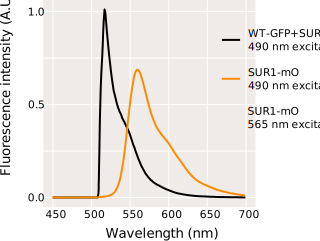
\includegraphics[width=\textwidth]{gfp_mo_spectra_1.pdf}
	\end{subfigure}
	\hfill
	\begin{subfigure}[t]{0.3\textwidth}
		\caption{}\label{ch6fig:wt_gfp_mo_spectra_1}
		\centering
		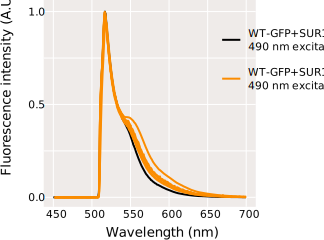
\includegraphics[width=\textwidth]{wt_gfp_mo_spectra_1.pdf}
	\end{subfigure}
	\hfill
	\begin{subfigure}[t]{0.3\textwidth}
		\caption{}\label{ch6fig:wt_gfp_mo_spectra_2}
		\centering
		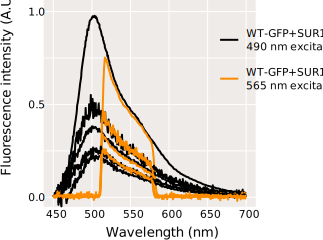
\includegraphics[width=\textwidth]{wt_gfp_mo_spectra_2.pdf}
	\end{subfigure}
	\vfill
	\begin{subfigure}[t]{0.3\textwidth}
		\caption{}\label{ch6fig:w311_gfp_mo_spectra_1}
		\centering
		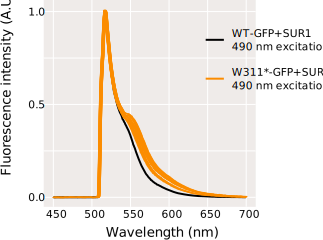
\includegraphics[width=\textwidth]{w311_gfp_mo_spectra_1.pdf}
	\end{subfigure}
	\hfill
	\begin{subfigure}[t]{0.3\textwidth}
		\caption{}\label{ch6fig:w311_gfp_mo_spectra_2}
		\centering
		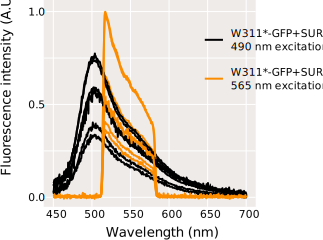
\includegraphics[width=\textwidth]{w311_gfp_mo_spectra_2.pdf}
	\end{subfigure}
	\hfill
	\begin{subfigure}[t]{0.3\textwidth}
		\caption{}\label{ch6fig:gfp_ofp_contrasts_1}
		\centering
		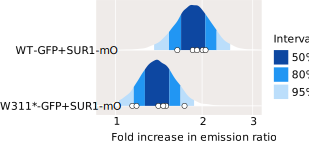
\includegraphics[width=\textwidth]{gfp_ofp_contrasts_1.pdf}
	\end{subfigure}
	\caption[SUR1-mO associates with WT-GFP and W311*-GFP]{
	\subref{ch6fig:gfp_mo_spectra_1} Averaged emission spectra of WT-GFP coexpressed with SUR1 in whole cells excited by \SI{490}{\nano\metre} light (black), overlayed by the averaged emission spectra of SUR1-m0 expressed in whole cells alone excited by \SI{490}{\nano\metre} light (orange) or \SI{565}{\nano\metre} light (pink).
	Spectra are shown normalised to the maximum fluorescence intensity.
	\subref{ch6fig:wt_gfp_mo_spectra_1}, \subref{ch6fig:wt_gfp_mo_spectra_2} Emission spectra from cells expressing WT-GFP+SUR1 (\subref{ch6fig:wt_gfp_mo_spectra_1}) or W311*-GFP+SUR1 (\subref{ch6fig:w311_gfp_mo_spectra_1}) excited by \SI{490}{\nano\metre} light (orange), with each spectra captured from a different cell.
	The idealised GFP emission spectrum from \subref{ch6fig:gfp_mo_spectra_1} is shown in black.
	Each spectra is normalised to the peak intensity of the GFP peak at \SI{508}{\nano\metre}.
	\subref{ch6fig:wt_gfp_mo_spectra_2}, \subref{ch6fig:wt_gfp_mo_spectra_2} The emission spectra from the previous panels (\subref{ch6fig:wt_gfp_mo_spectra_1} and \subref{ch6fig:wt_gfp_mo_spectra_2} respectively) with the idealised GFP peak subtracted are shown in black.
	Overlayed in orange are the emission spectra from the same cells when excited with \SI{565}{\nano\metre} light.
	\subref{ch6fig:gfp_ofp_contrasts_1} The increase in emission ratio is the diffence between the fluorescence intensity of SUR1-mO expressed alone when excited by \SI{490}{\nano\metre} or \SI{565}{\nano\metre} light, and the fluorescence intensity of SUR1-mO coexpressed with either of the GFP labelled constructs when excited by \SI{490}{\nano\metre} or \SI{565}{\nano\metre} light.
	The ratio for each cell is shown as a circle.
	The posterior probability distribution for the fold increase in emission ratio is shown coloured by its intervals for each construct separately.
	}\label{ch6fig:sur_assays}
\end{figure}

\subsection{Presence of SUR1-TMD0 alone does not dramatically alter nucleotide binding}

We sought to clarify the role of the TMD0 and L0 regions of SUR1 in binding to the inhibitory nucleotide binding site of Kir6.2.
We used two SUR1 truncation constructs; TMD0 consisting of the N-terminal 1-195 residues of SUR1, and TMD0-L0 consisting of the N-terminal 1-232 residues of SUR1.
Firstly, we established whether these constructs were capable of supporting trafficking and expression at the cell membrane as previously reported \ref{babenko_sur_2003-1, chan_n-terminal_2003-1}.
In our luminesence based cell-surface expression assay, we found that TMD0 and TMD0-L0 increased the expression of WT-GFP approximately 3-fold over the expression of WT-GFP alone (Figure \ref{ch6fig:tmd0s_surface_expression_1}, \ref{ch6fig:tmd0s_surface_expression_2}).
This level of expression is somewhat less than observed for full-length SUR1.
However, when we coexpressed either TMD0 or TMD0-L0 with W311*-GFP, we found less evidence to suggest an increase of surface expression when compared to expression of W311*-GFP alone (Figure \ref{ch6fig:tmd0s_surface_expression_1}, \ref{ch6fig:tmd0s_surface_expression_3});
i.e., our posterior probability distributions for the fold increase in expression overlapped 1.
Indeed, when we attempted to excise patches coexpressing W311*-GFP and either TMD0 or TMD0-L0, we were unable to detect channel currents, while we were able to measure \si{\nano\ampere} currents from WT-GFP coexpressed with TMD0 or TMD0-L0.

Despite being unable to detect channel currents, as with W311*-GFP expressed alone, we were able to detect ANAP and GFP fluorescence from unroofed membrane patches coexpressing W311*-GFP with either TMD0 or TMD0-L0.
To determine whether this fluorescence was emitted from W311*-GFP correctly coassembled with the truncated SUR1 constructs, we measured the emission ratio of TMD0-L0 labelled at the C-terminus with mOrange (TMD0-L0-mO) as described previously.
We coexpressed either WT-GFP or W311*-GFP with TMD0-L0-mO and measured the emission ratio of directly excited mOrange to indirectly excited mOrange in whole cells (Figure \ref{ch6fig:gfp_ofp_contrasts_2}).
For WT-GFP+TMD0-L0-mO, we observed an increase in emission ratio over TMD0-L0-mO of a similar magnitude for the increase observed for WT-GFP+SUR1-mO (Figure \ref{ch6fig:gfp_ofp_contrasts_1}).
This is consistent with TMD0-L0-mO coassembling with WT-GFP in unroofed membanes, as an increase in emission ratio requires the two fluorophores to be in close proximity.
However, coexpression of W311*-GFP and TMD0-L0-mO resulted in an emission ratio with a posterior probability distribution which overlaps 1; i.e. there is little evidence to suggest there is an increase in the emission ratio.
Again, this may be due to decreased expression of W311*-GFP compared to WT-GFP, but we cannot discount the possibility that we are measuring from a heterogenous population of W311*-GFP channels and W311*-GFP+TMD0-L0 channels.

\begin{figure}[h]
	\centering
	\begin{subfigure}[t]{0.45\textwidth}
		\caption{}\label{ch6fig:tmd0s_surface_expression_1}
		\centering
		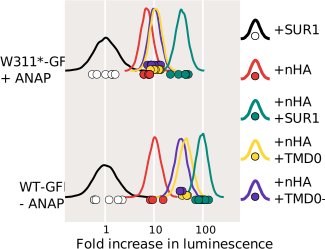
\includegraphics[width=\textwidth]{tmd0s_surface_expression_1.pdf}
	\end{subfigure}
	\hfill
	\begin{subfigure}[t]{0.45\textwidth}
		\caption{}\label{ch6fig:tmd0s_surface_expression_2}
		\centering
		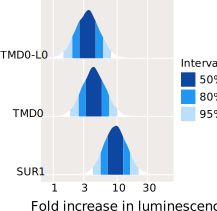
\includegraphics[width=\textwidth]{tmd0s_surface_expression_3.pdf}
	\end{subfigure}
	\vfill
	\begin{subfigure}[t]{0.45\textwidth}
		\caption{}\label{ch6fig:tmd0s_surface_expression_2}
		\centering
		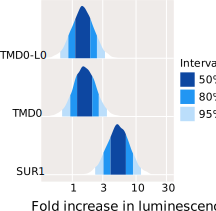
\includegraphics[width=\textwidth]{tmd0s_surface_expression_2.pdf}
	\end{subfigure}
	\hfill
	\begin{subfigure}[t]{0.45\textwidth}
		\caption{}\label{ch6fig:gfp_ofp_contrasts_2}
		\centering
		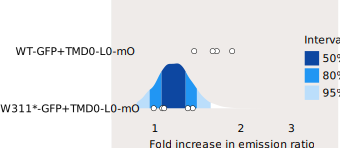
\includegraphics[width=\textwidth]{gfp_ofp_contrasts_2.pdf}
	\end{subfigure}
	\caption[TMD0 and TMD0-LO associate with WT-GFP and W311*-GFP]{
	\subref{ch6fig:tmd0s_surface_expression_1} Individual observations (points) and posterior probability distributions for surface expression of Kir6.2 constructs in the presence of SUR1 (blue), TMD0 (orange), TMD0-L0 (brown) or alone (red).
	Before fitting, the observations for each construct were centered by subtracting the mean of the luminesence observed without the N-terminal HA tag.
	\subref{ch6fig:tmd0s_surface_expression_2}, \subref{ch6fig:tmd0s_surface_expression_3} Contrasts between WT-GFP (\subref{ch6fig:tmd0s_surface_expression_2}) or W311*-GFP (\subref{ch6fig:tmd0s_surface_expression_2}) surface expression when coexpressed with SUR1, TMD0 or TMD0-L0 and WT-GFP alone.
	Contrasts are expressed as a fold increase in luminescence, so that a value of 1 means expression is the same as WT-GFP or W311*-GFP alone.
	Different intervals in the posterior probability distribution of the contrasts are shown in shades of blue.
	\subref{ch6fig:gfp_ofp_contrasts_2}  Contrasts in emission ratios between direct excitation of TMD0-L0-mO and excitation of WT-GFP or W311*-GFP coexpressed with TMD0-L0-mO in whole cells.
	Contrasts are expressed as a fold increase in emision ratio, so that a value of 1 means the ratio is the same as the emission ratio of TMD0-L0-mO expressed alone.
	Different intervals in the posterior probability distribution of the contrasts are shown in shades of blue.
	}\label{ch6fig:tmd0_assays}
\end{figure}

We coexpressed either TMD0 or TMD0-L0 in combination with W311*-GFP and measured TNP-ATP binding in unroofed membranes (Figure \ref{ch6fig:tmd0s_unroofed_1}).
We found that the data were not particularly distinguishable from that collected from TNP-ATP binding to W311*-GFP expressed alone; although this may be due to measuring from a mixed population of channels.
To confirm that we could replicate the functional effects of TMD0-L0 on Kir6.2, we measured currents frome excised patches expressing WT-GFP+TMD0-L0 and measured inhibition by ATP (Figure \ref{ch6fig:tmd0_atp_trace}).
Similarly to \citeauthor{babenko_sur_2003-1} and \citeauthor{chan_n-terminal_2003-1}, we observed a decrease in sensitivity to nucleotide inhibition in channels formed from WT-GFP and TMD0-L0 to channels formed from WT-GFP alone (Figure \ref{ch6fig:tmd0_atp_1}).

\begin{figure}[h]
	\centering
	\begin{subfigure}[t]{0.45\textwidth}
		\caption{}\label{ch6fig:tmd0s_unroofed_1}
		\centering
		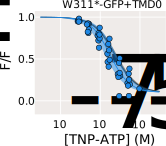
\includegraphics[width=\textwidth]{tmd0s_unroofed_1.pdf}
	\end{subfigure}
	\hfill
	\begin{subfigure}[t]{0.22\textwidth}
		\caption{}\label{ch6fig:tmd0_atp_trace}
		\centering
		
\includegraphics[width=\textwidth]{tmd0_atp_trace.pdf}
	\end{subfigure}
	\hfill
	\begin{subfigure}[t]{0.22\textwidth}
		\caption{}\label{ch6fig:tmd0_atp_1}
		\centering
		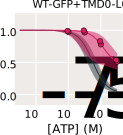
\includegraphics[width=\textwidth]{tmd0_atp_1.pdf}
	\end{subfigure}
	\vfill
	\begin{subfigure}[t]{0.9\textwidth}
		\caption{}\label{ch6fig:tmd0s_ec50s}
		\centering
		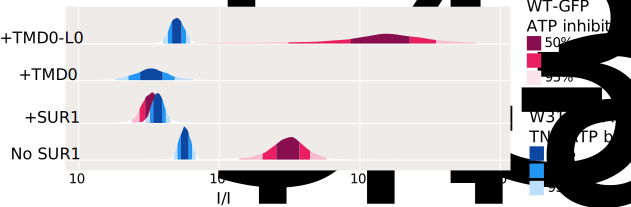
\includegraphics[width=\textwidth]{tmd0s_ec50s.pdf}
	\end{subfigure}
	\caption[TMD0 and TMD0-LO subtly alter binding to Kir6.2]{
	\subref{ch6fig:tmd0s_unroofed_1} Fluorescence quenching of W311*-GFP expressed with TMD0 (left) or TMD0-L0 (right) by TNP-ATP in unroofed membrane patches is shown in orange.
	Each point represents an individual experiment.
	The smooth filled curves are the \SI{95}{\percent} intervals of the posterior probability distribution of fits to equation \ref{eq:hill} as described in the methods.
	The blue curve is the fit to the W311*-GFP expressed alone fluorescence quenching by TNP-ATP and is shown for comparison.
	\subref{ch6fig:tmd0_atp_trace} Current inhibition by ATP from an excised patch expressing WT-GFP+TMD0-L0.
	The concentration of ATP perfused is shown by colour.
	The zero-current level is indicated as a dotted line.
	\subref{ch6fig:tmd0_atp_1} Current inhibition of WT-GFP+TMD0-L0 in excised patches by ATP is shown in orange.
	The smooth filled curves are the \SI{95}{\percent} intervals of the posterior probability distribution of fits to equation \ref{eq:hill} as described in the methods.
	The blue curve is the fit to the WT-GFP expressed alone current inhibition by ATP and is shown for comparison.
	\subref{ch6fig:tmd0s_ec50s} Posterior probability distributions for the estimated population $IC_{50}$ or $EC_{50}$ values are shown in purple ($IC_{50}$ for ATP inhibition of WT-GFP) or blue ($EC_{50}$ for TNP-ATP binding to W311*-GFP in unroofed membranes).
	Each distribution is shaded with respect to its intervals.
	}\label{ch6fig:tmd0_binding}
\end{figure}

\section{SUR1 and nucleotide regulation}

\subsection{Mutations at SUR-K205 alter nucleotide binding and inhibition}

Residue K205 of SUR1 is located in the L0 region which links TMD0 and TMD1.
While expression of Kir6.2 and TMD0-L0 have shown that the region is important in modulating the $P_O$ of K\ATP{} channels \cite{babenko_sur_2003, chan_n-terminal_2003-1, pratt_n-terminal_2011}, it does not confer the high sensitivity to ATP inhibition seen in Kir6.2+SUR1 channels.
It has therefore been suggested that the elements of SUR1 which contribute to the higher sensitivity of K\ATP{} channels to ATP inhibition lie outside of this region \cite{babenko_sur_2003, pratt_engineered_2012-1}.
However, the cryo-EM structures of K\ATP{} suggest a close proximity between L0 and the ATP binding pocket \cite{martin_anti-diabetic_2017-1, lee_molecular_2017-1, li_structure_2017} and mutations in this region reduce the sensitivity of K\ATP{} to nucleotide inhibition \cite{ding_structural_2019,pratt_engineered_2012-1, masia_mutation_2007}.
Mutation of K205 to A \cite{ding_structural_2019} or E \cite{pratt_engineered_2012} have resulted in marked reduction of K\ATP{} channel sensitivity to nucleotide inhibition.

We excised patches expressing W311*-GFP+SUR1-K205A or W311*-GFP+SUR1-K205E and measured current inhibition and fluorescence quenching by TNP-ATP simultaneously.
We found that both substitutions resulted in an increased IC\textsubscript{50} for TNP-ATP inhibition and an increased EC\textsubscript{50} for TNP-ATP binding, with K205E exhibiting a more pronounced effect than K205A.
Fitting the data to our MWC model gave parameter estimates for $K_A$ which were reduced when compared to wild-type SUR1; with the neutral mutation K205A not affecting $K_A$ quite as much as the charge reversal mutation K205E.
In addition, both mutations led to similar increases in $D_A$.
Thus, the reduced sensitivity to nucleotide inhibition is due to a combination of reduced apparent binding affinity in addition to reduced stabilisation of the closed state of the channel by nucleotides. 

\begin{figure}[h]
	\centering
	\begin{subfigure}[t]{0.45\textwidth}
		\caption{}\label{ch6fig:k205_1}
		\centering
		\includegraphics[width=\textwidth]{k205_1.pdf}
	\end{subfigure}
	\hfill
	\begin{subfigure}[t]{0.45\textwidth}
		\caption{}\label{ch6fig:k205_2}
		\centering
		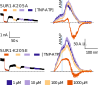
\includegraphics[width=\textwidth]{k205_2.pdf}
	\end{subfigure}
	\vfill
	\begin{subfigure}[t]{0.45\textwidth}
		\caption{}\label{ch6fig:k205_3}
		\centering
		\includegraphics[width=\textwidth]{k205_3.pdf}
	\end{subfigure}
	\hfill
	\begin{subfigure}[t]{0.45\textwidth}
		\caption{}\label{ch6fig:k205_4}
		\centering
		\includegraphics[width=\textwidth]{k205_4.pdf}
	\end{subfigure}
	\vfill
	\begin{subfigure}[t]{0.9\textwidth}
		\caption{}\label{ch6fig:k205_5}
		\centering
		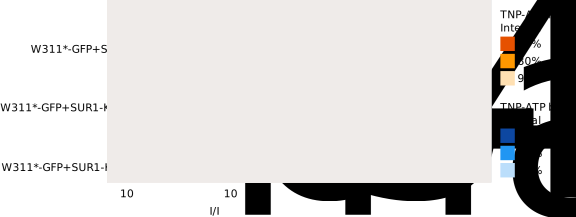
\includegraphics[width=\textwidth]{k205_5.pdf}
	\end{subfigure}
	\caption[Functional effects of mutations at K205]{
	\subref{ch6fig:k205_1} Residue K205 is shown in purple in the cryo-EM structure of K\ATP{} (PDB \#6C3P).
	Adjacent subunits of Kir6.2 are shown in two different shades of yellow, TMD0 and L0 of SUR1 are shown in two different shades of blue.
	The core of SUR1 is not shown.
	Bound ATP is shown in red.
	\subref{ch6fig:k205_2} Current inhibition (left) and fluorescence quenching (right) from an excised patch expressing W311*-GFP+SUR1-K205A (upper) or W311*-GFP+SUR1-K205E (lower).
	The concentration of TNP-ATP perfused is shown by colour.
	The location of the peak ANAP fluorescence is marked as a grey box.
	\subref{ch6fig:k205_3}, \subref{ch6fig:k205_4} Current inhibition (\subref{ch6fig:k205_3}) and fluorescence quenching (\subref{ch6fig:k205_4}) of K205 mutants in the W311*-GFP+SUR1 background by TNP-ATP acquired simultaneously in excised patches.
	Each point represents an individual experiment.
	The smooth filled curves are the \SI{95}{\percent} intervals of the posterior probability distribution of fits to equation \ref{eq:hill} as described in the methods.
	\subref{ch6fig:k205_4} Posterior probability distributions for the estimated population $IC_{50}$ or $EC_{50}$ values are shown in orange ($IC_{50}$ for TNP-ATP inhibition) or blue ($EC_{50}$ for TNP-ATP binding).
	Each distribution is shaded with respect to its intervals.
	}\label{ch6fig:k205_fig1}
\end{figure}

\begin{figure}[h]
	\centering
	\begin{subfigure}[t]{0.9\textwidth}
		\caption{}\label{ch6fig:mwc_k205_1}
		\centering
		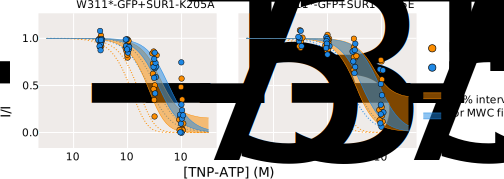
\includegraphics[width=\textwidth]{mwc_k205_1.pdf}
	\end{subfigure}
	\vfill
	\begin{subfigure}[t]{0.9\textwidth}
		\caption{}\label{ch6fig:mwc_k205_2}
		\centering
		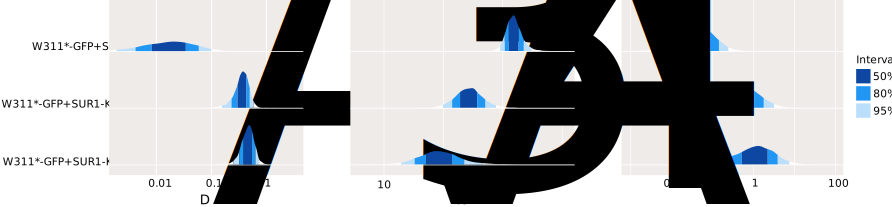
\includegraphics[width=\textwidth]{mwc_k205_2.pdf}
	\end{subfigure}
	\caption[K205 mutations affect gating and nucleotide binding]{
	\subref{ch6fig:mwc_k205_1} Current inhibition (orange) and fluorescence quenching (blue) from excised patches expressing W311*-GFP+SUR1-K205A (left) or W311*-GFP+SUR1-K205E (right).
	The smooth filled curves are the \SI{95}{\percent} intervals of the posterior probability distribution of fits to equations \ref{eq:mwc_binding} and \ref{eq:normalised_po}.
	Dashed curves are for comparison, and indicate the \SI{95}{\percent} intervals of the posterior probability distribution of fits to equations \ref{eq:mwc_binding} and \ref{eq:normalised_po} for the W311*-GFP+SUR1 data.
	\subref{ch6fig:mwc_k205_2} Posterior probability distributions for the estimated population $L$, $D$ and $K_A$ parameters from the fits in panel \subref{ch6fig:mwc_k205_1}.
	Each distribution is shaded with respect to its intervals.
	}\label{ch6fig:k205_fig2}
\end{figure}

\section{Discussion}

Expression of W311*-GFP in the absence of SUR1 reduces the apparent nucleotide binding affinity by only a small amount in unroofed membranes; approxiamtely 2-fold.
This is in contrast to the dramatic 10-fold reduction in sensitivity to inhibition by ATP observed when WT-GFP is expressed in the absence of SUR1.
We also found that coexpression of W311*-GFP with TMD0 or TMD0-L0 did not result in an increase in apparent nucleotide binding affinity, although this finding is caveated by the possible mixture of correctly complexed mini-K\ATP{} channels and W311*-GFP subunits alone in the unroofed membranes.

Despite these somewhat inconclusive findings, we saw a clear effect of mutating residue K205 in the L0 loop of SUR1.
Similar to the findings of \citeauthor{ding_structural_2019}, we observed a marked reduction in sensitivity to TNP-ATP inhibition when the residue was mutated to an alanine, and a further reduction when it was mutated to glutamic acid.
Fitting the data to the MWC model reveals that the reduction in sensitivity is due to both a reduction in the microscopic binding affinity for TNP-ATP, and a decrease in the transduction of nucleotide binding to channel closure.

The structure of K205 resolved by \citeauthor{ding_structural_2019} suggested that the long, positively charged side chain directly coordinates the \textgreek{b}- and \textgreek{g}-phosphates of bound ATP \cite{ding_structural_2019}.
Our results are consistent with the hypothesis that mutation to an alanine, thus removing the positive charge, directly disrupts nucleotide binding.
We also observe a further reduction in the microscopic binding affinity upon substitution by glutamic acid, which has a long and negatively charged side chain.
Again, this is consistent with the idea that K205 directly coordinates the negatively charged phosphates of ATP, and explains the reduction in sensitivity to ATP inhibition observed by \citeauthor{pratt_engineered_2012} when they made the same mutation.

Our MWC fits also suggest that mutation of K205 reduces the ability of nucleotides to close the channel.
As we calculated for the C166S mutation in Kir6.2, we can express this reduction in terms of the free energy contributed to the conformational change of closure.
For the SUR1-K205A construct, the free energy is \SIrange{5.6}{18.3}{\kilo\joule\per\Molar},and for the SUR1-K205E construct, the free energy is \SIrange{3.3}{13.9}{\kilo\joule\per\Molar}, much reduced from that of wild-type SUR1 which is \SIrange{23.0}{63.4}{\kilo\joule\per\Molar}.
This suggests that the positive charge K205 contributes to the inhibitory binding site is important for transduction of nucleotide binding to channel closure.

This finding does not explain why TMD0-L0 expression alone is not enough to restore full-length SUR1 like nucleotide inhibition.
Coexpression of TMD0-L0 with WT-GFP exhibits decreased sensitivity to nucleotide inhibition when compared to full length SUR1, as seen in previous studies \cite{babenko_sur_2003, chan_n-terminal_2003-1, pratt_n-terminal_2011}.
Our findings are consistent with the hypothesis that the elements of the L0 linker which enhance the binding affinity of nucleotides for Kir6.2 and which increase the intrinsic open probability of the K\ATP{} channel are separate; and also suggest that the linker plays an active role in transducing binding to closure.
